\documentclass{beamer}

% Some common packages
\usepackage{graphicx, color}
\usepackage{alltt}
\usepackage{booktabs, calc, rotating}
\usepackage[round]{natbib}
\usepackage{multicol}
\usepackage{amsmath, amsbsy, amssymb, amsthm, graphicx}
\usepackage[english]{babel}
\usepackage{xkeyval} 
\usepackage{xfrac}
\usepackage[normalem]{ulem}
\usepackage{fancyvrb} 
\usepackage{tikz, geometry, tkz-graph, xcolor}
\usepackage[latin1]{inputenc}
\usepackage{times}
\usepackage[T1]{fontenc}

% Shortcuts
\newcommand{\empr}[1]{{\emph{\color{red}#1}}}
\newcommand{\cov}{\mathrm{cov}}
\newcommand{\pkg}[1]{{\textbf{\texttt{#1}}}}
\newcommand{\dif}{\mathrm{d}}
\newcommand{\bigbrk}{\vspace*{2in}}
\newcommand{\smallbrk}{\vspace*{.1in}}
\newcommand{\midbrk}{\vspace*{1in}}
\newcommand{\red}[1]{{\color{red}#1}}
\newcommand{\blue}[1]{{\color{blue}#1}}
\newcommand{\green}[1]{{\color{green}#1}}
\newcommand{\calc}[1]{{\fbox{\mbox{#1}}}}
\newcommand{\Var}{\mathrm{Var}}%
\newcommand{\Cov}{\mathrm{Cov}}%

\mode<presentation>
{
  \usetheme{UTD}
  \usecolortheme[RGB={200,0,0}]{structure}
  \setbeamercovered{transparent}
}

% fancy for Verbatim?
\fvset{frame=single,framesep=1mm,fontfamily=courier,fontsize=\scriptsize,numbers=left,framerule=.3mm,numbersep=1mm,commandchars=\\\{\}}


\title[Survival Analysis]{Applied Survival Analysis Using R\\ Chapter 2: Basic Principle of Survival Analysis}
\author[Qi Guo]{Qi Guo}
\institute[UTD]{Department of Mathematical Sciences \\ 
The University of Texas at Dallas}
\date{April, 9 2019}
	


\begin{document}

\begin{frame}
  \titlepage
\end{frame}

% Set up UTD backgroud
\setbeamercolor*{item}{fg=red}
\bgroup
\usebackgroundtemplate{
\tikz[overlay,remember picture] \node[opacity=0.05, at=(current page.center)] {
   
\includegraphics[height=\paperheight,width=\paperwidth]{UTDbg}};}


\section[Outline]{}
\begin{frame}
  \tableofcontents
\end{frame}

\section{Two key ways of specifying a survival analysis}
\begin{frame}
\frametitle{The Hazard and Survival Functions}
\begin{defblock}{The Survival Function}
	Survival analysis is defines the probability of surviving up to a point $t$. Formally,\linebreak \centerline{$S(t) = 1 - P (T\le t) = 1 - F(t),\   0<t<\infty$} \linebreak And it decreases over time
\end{defblock}

\begin{defblock}{The Hazard Function}
	It is the {\color{red} instantaneous failure rate}. It is the probability that, given that a subject has survived up to time t, he or she fails in the next small interval of time, divided by the length of that interval. Formally,\linebreak \centerline{
		$h(t) =  \lim\limits_{\delta\to0}\frac{P(t\le T < t + \delta|T\ge t)}{\delta}.$
		}
\end{defblock}
\end{frame}

\section{Connections}
\begin{frame}
\frametitle{Connections}
\begin{itemize}
\item Cumulative risk function: $F(t) =  P (T\le t),\   0<t<\infty$
\item Probability density function: $f(t) = \frac{\dif F(t)}{\dif t} =  - \frac{\dif S(t)}{\dif t}$
\item So we can deduce the following two formulas:
\begin{itemize}
	\item $h(t) = \frac{f(t)}{S(t)} $
	\item $H(t) = \int_{0}^{t} h(u) du$ 
	\item $S(t) = exp(- \int_{0}^{t} h(u) du) = exp(-H(t))$
	\end{itemize}
\end{itemize}
\end{frame}


\section{Mean and Median Survival Time}
\begin{frame}
\frametitle{Mean and Median Survival Time}
\begin{itemize}	
\item The {\color{red}mean} survival is the expected value of the survival time \linebreak
\centerline{$\mu = E(T) =\int_{0}^{\infty} tf(t) dt $}

\item or \linebreak
\centerline{$\mu =\int_{0}^{\infty} S(t) dt $}

\item The mean survival also cannot be computed with the {\color{red}Kaplan-Meier survival curve} when the curve does not reach zero, an issue we will discuss in the next chapter.

\item The median survival time is defined as the time t such that $S(t) = 1/2$
\end{itemize}
\end{frame}


\section{Parametric Survival Distributions}
\begin{frame}
\frametitle{Exponential Distribution }
\begin{itemize}
\item When modeling human or animal survival, it is hard to know what parametric family to choose, and often none of the available families has sufficient flexibility to model the actual shape of the distribution, so commonly we analyze the \empr{non-parametric survival distribution} due to more \empr{flexible} and \empr{applicable}.
\item The exponential distribution is the simplest but classical survival distribution, has a \empr{constant} hazard, {\color{red} $h(t)=\lambda$}
\item \empr{$H(t)=\lambda t$}
\item \empr{$S(t)=e ^{-H(t)}=e^{-\lambda t}$}
\item \empr{$f(t)=S(t)h(t)=\lambda e^{-\lambda t}$}
\item $E(T) = 1/ \lambda$
\item $t_{med} = log(2)/\lambda$

\end{itemize}
\end{frame}

\pagebreak
\begin{frame}
\frametitle{Weibull Distribution }
\begin{itemize}
	\item The exponential distribution is easy to work with, but the constant hazard assumption is not often appropriate for describing the lifetimes of humans or animals.
	\item \empr{$h(t)=\alpha\lambda^{\alpha}t^{\alpha-1}$}
	\item \empr{$H(t)=(\lambda t)^{\alpha}$}
	\item \empr{$S(t)=e ^{-(\lambda t)^{\alpha}}$}
	\item $E(T) = \frac{\Gamma(1+1/\alpha)}{\lambda}$
	\item $t_{med} = \frac{[log(2)]^{1/\alpha}}{\lambda}$	
\end{itemize}
\end{frame}

\pagebreak
\begin{frame}[fragile]
\frametitle{In R}
\begin{itemize}	
	\item We may generate random variables from the exponential or Weibull distribution using the functions ``\pkg{rexp}'' and``\pkg{rweib}''.
	\item The functions ``\pkg{dweibull}'' and ``\pkg{pweibull}'' compute the p.d.f. and c.d.f., respectively, of the Weibull distribution.
	\item These functions use the arguments ``{\color{red}shape}'' and ``{\color{red}scale}'' to represent the parameters $\alpha$ and $1/\lambda$.
	
\begin{Verbatim}
> tt.weib <- rweibull(1000, shape=1.5, scale=1/0.03)
> mean(tt.weib)
[1] 31.35497
> median(tt.weib)
[1] 26.84281
\end{Verbatim}

\end{itemize}
\end{frame}

\pagebreak
\begin{frame}[fragile]
\frametitle{In R}
\begin{itemize}	
\item Plot the \empr{Weibull survival function} with  
$\alpha=1.5$ and \linebreak $\lambda=0.03$ by first defining a function ``\pkg{weibSurv}'' with these parameters and then using the ``\pkg{curve}'' function to plot the curve as follows:
\begin{Verbatim}
> weibSurv <- function(t, shape, scale) pweibull(t, shape=shape, 
scale=scale, lower.tail=F)
> curve(weibSurv(x, shape=1.5, scale=1/0.03), from=0, to=80, 
ylim=c(0,1), ylab='Survival probability', xlab='Time')
\end{Verbatim}
\item Plot the \empr{hazard function} with  
p.d.f. divided by the survival function:
\begin{Verbatim}
> weibHaz <- function(x, shape, scale) dweibull(x, shape=shape, 
scale=scale)/pweibull(x, shape=shape, scale=scale,
lower.tail=F)
> curve(weibHaz(x, shape=1.5, scale=1/0.03), from=0, to=80,
ylab='Hazard', xlab='Time', col="red")
\end{Verbatim}
\end{itemize}
\end{frame}

\pagebreak
\begin{frame}[fragile]
\frametitle{In R}
\begin{itemize}	
\item The other two curves obtained using $\alpha=1$ and $\alpha=0.75$ when calling the ``\pkg{curve}''  function. To place the additional curves on the plot, add ``\pkg{add=T}''  as an option to the ``\pkg{curve}''  function.
\begin{Verbatim}
> curve(weibHaz(x, shape=1, scale=1/0.03), from=0, to=80,
ylab='Hazard', xlab='Time', col="black", add = TRUE)
> curve(weibHaz(x, shape=0.75, scale=1/0.03), from=0, to=80,
ylab='Hazard', xlab='Time', col="blue", add = TRUE)
\end{Verbatim}

\begin{figure}
	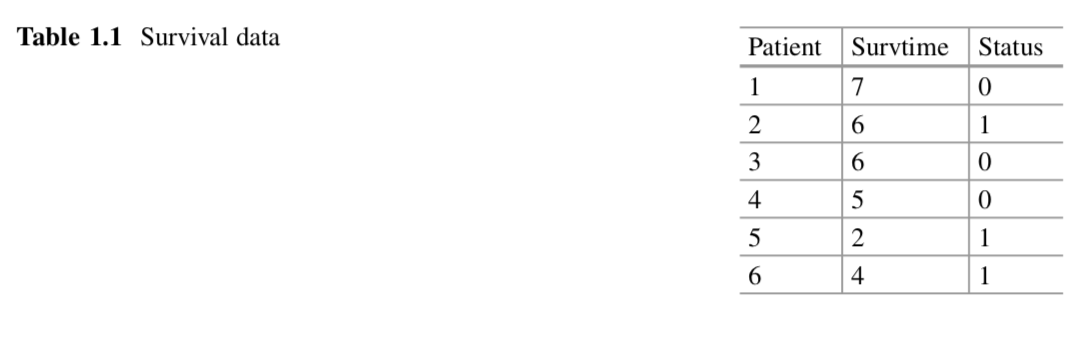
\includegraphics[scale = .4]{001.png}
\end{figure}
\end{itemize}
\end{frame}

\section{A Brief Introduction to Maximum Likelihood Estimation}
\begin{frame}
\frametitle{M.L.E}
\begin{itemize}	
\item No Censoring	\linebreak
 $L(\lambda; t_1, t_2,...,t_n) = f(t_1,\lambda)\cdot f(t_2,\lambda)\cdot\cdots\cdot f(t_n,\lambda)= \prod\limits_{i=1}^{n} f(t_i,\lambda)$
\end{itemize}

\begin{itemize}	
\item Right-censoring
$L(\lambda; t_1, t_2,...,t_n) = \prod\limits_{i=1}^{n} f(t_i,\lambda)^{\delta_i}\cdot S(t_i,\lambda)^{1-\delta_i}= \prod\limits_{i=1}^{n}h(t_i,\lambda)^{\delta_i}\cdot S(t_i,\lambda)$
\end{itemize}
\begin{itemize}	
\item This expression means that when $t_i$ is an \empr{observed death}, the censoring indicator is \empr{$\delta_i = 1$}, and we enter a \empr{p.d.f. factor}. When $t_i$ is a \empr{censored observation}, we have \empr{$\delta_i = 0$} we enter a \empr{survival factor}. 
\end{itemize}
\end{frame}

\pagebreak
\begin{frame}
\frametitle{Example}
\begin{itemize}	
\item Exponential M.L.E	\linebreak $L(\lambda) =  \prod\limits_{i=1}^{n}[\lambda e^{-t_i /\lambda}]^{\delta_i}[e^{-\lambda t_i}]^{1-\delta_i} $ \linebreak
$d = \sum\limits_{i=1}^{n}\delta_i$,means the total of the death\linebreak
$V = \sum\limits_{i=1}^{n}t_i$,means the total of the time of patients on study
\end{itemize}
\begin{itemize}
\item Log-Likelihood\linebreak	
 $\ell(\lambda) = d\ log\lambda - \lambda V$
\end{itemize}
\begin{itemize}	
\item First Derivative(\empr{Score Function})\linebreak
$\ell^{'}(\lambda) = \frac{d}{\lambda} -  V$ $\Rightarrow$ $\hat{\lambda} = \frac{d}{V}$
\end{itemize}
\end{frame}

\pagebreak
\begin{frame}
\frametitle{Example}
\begin{itemize}	
\item Second Derivative(\empr{Information})\linebreak$\ell^{''}(\lambda) = -\frac{d}{\lambda^{2}} = -I(\lambda)$
\end{itemize}
\begin{itemize}	
\item The inverse of the (\empr{Information}) is approximately the variance of the m.l.e \linebreak$var(\hat{\lambda})\approx I^{-1}(\lambda)= \lambda^{2}/d$
\end{itemize}
\begin{itemize}	
\item Substitute the $\hat{\lambda}$ for $\lambda$ to obtain the observed information $I(\hat{\lambda})$, and get an estimate of the variance \linebreak
$\hat{var}(\hat{\lambda})\approx I^{-1}(\hat{\lambda})= \hat{\lambda}^{2}/d=d/V^{2}$
\end{itemize}
\begin{itemize}	
\item Use this formula to carry out hypothesis tests or find a confidence interval for $\lambda$.
\end{itemize}
\end{frame}

\end{document}

